\documentclass[a4paper, 11pt]{article}

\usepackage[UTF8]{ctex}
\usepackage{amsmath}
\usepackage{xfrac}
\usepackage{geometry}
\usepackage{fancyhdr}
\usepackage{lastpage}
\usepackage{minted}
\usepackage{fontspec}
\usepackage{graphicx}
\usepackage{adjustbox}
\usepackage{tabularx}
\usepackage{multirow}
\usepackage{dblfloatfix}
\usepackage{hyperref}
\usepackage{wrapfig}
\usepackage{float}
\usepackage{caption}

% 设置页面
\geometry{hmargin=3.18cm, vmargin=2.54cm} % 页边距
\pagestyle{fancy}
\fancyhf{}
\chead{常州大学实验报告} % 页眉
\renewcommand{\headwidth}{\textwidth} % 页眉分割横线
\cfoot{第 \thepage 页,共 \pageref{LastPage} 页} % 页脚,显示页码

% 设置字体
\setmainfont{Times New Roman}
\setsansfont{Arial}
\setCJKsansfont{Microsoft YaHei}
\setmonofont[Scale=0.95]{Consolas}
\setCJKmonofont[Scale=0.95]{Microsoft YaHei}

% 设置代码
\setminted{autogobble, baselinestretch=1, breaklines, frame=lines, framesep=4mm, linenos, style=vs, stripnl, tabsize=4}
\newfloat{snippet}{p}{}
\floatname{snippet}{代码片段}
\newmintedfile[cppfile]{cpp}{}
\newcommand{\codeinline}{\mintinline{text}}

% 设置目录
\graphicspath{ {images/} }

% 设置表格
\newcolumntype{C}{>{\centering\arraybackslash}X}

\begin{document}

% 封面
\begin{titlepage}

	\begin{center}
		\marginbox{0cm 0cm 0cm 3cm}{
			
\includegraphics[width=2.67cm, height=2.67cm]{logo.png}
			\marginbox{2cm 0cm 0cm 0cm}{
\includegraphics[height=2.67cm]{logo2}}
		}
		\marginbox{0cm 0cm 0cm 3cm}{
			\fontsize{42pt}{0}\selectfont
			实 \enspace 习 \enspace 报 \enspace 告
		}
	\end{center}

	\begin{table}[!b]
		\fontsize{14pt}{0}\selectfont
		\begin{tabularx}{\textwidth}{lClC}
			\rule{0pt}{36pt}
			题  目 & \multicolumn{3}{c}{字符界面小游戏——鲲宠大乐斗}                           \\
			\cline{2-4}
			\rule{0pt}{36pt}
			学  院 & \multicolumn{3}{c}{信息数理学院}                                         \\
			\cline{2-4}
			\rule{0pt}{36pt}
			专业班级 & \multicolumn{3}{c}{物联网 161}                                           \\
			\cline{2-4}
			\rule{0pt}{36pt}
			学生姓名 & \multicolumn{3}{c}{钱宇超}                                               \\
			\cline{2-4}
			\rule{0pt}{36pt}
			学  号 & \multicolumn{3}{c}{15488122}                                             \\
			\cline{2-4}
			\rule{0pt}{36pt}
			指导老师 & \multicolumn{3}{c}{陈哲}                                                 \\
			\cline{2-4}
			\rule{0pt}{36pt}
			实习时间 & 2018 年 5 月 21 日                             & ~ & 2018 年 5 月 25 日 \\
			\cline{2-2} \cline{4-4}
			\rule{0pt}{36pt}
		\end{tabularx}
	\end{table}

\end{titlepage}

% 目录页
\tableofcontents
\clearpage

\section{实习目的}

利用已有的 C 语言知识,进一步学习 Windows API 相关知识,通过编写一个字符界面小游戏来实践 C 语言在 Windows 下的开发过程,学习使用 Windows API 中操作控制台的相关接口,例如 \codeinline{GetConsoleCursorInfo}、\codeinline{SetConsoleCursorPosition}、\codeinline{WriteConsole} 等,同时体会开发软件时「解耦」的设计理念,熟悉各模块分离的软件架构方式,以及体验\textbf{团队分工}形式的软件开发流程。

\section{实习内容}

\subsection{问题分析和操作逻辑设计}

综合根据实训课教学代码的实现和自身对该游戏的理解,小游戏启动后需经过一个加载界面(由于只是实习目的,这里实际并不需要加载游戏内容,而是仅仅显示一个加载动画),持续若干秒后启动到游戏主菜单,这里会进入一个键盘事件循环,不断尝试读取用户的键盘输入,一旦有输入,就根据键码来执行不同的操作,如按下「下方向键」会高亮下一个菜单项、按下回车会选中菜单项。用户在主菜单按下回车或空格后,会根据菜单项的不同进入不同的次级菜单,或进入其它界面,在次级菜单中也同样有键盘事件循环,操作逻辑和主菜单相似。

为了保持界面的一致性和开发的便捷性,在不影响实践效果的情况下,决定将主要的游戏界面也设计为和主菜单类似的样式,也就是说,游戏的功能也通过菜单的形式让用户选择,设想的游戏方式类似于网络上的一款 HTML5 小游戏——\href{http://catx.me/adarkroom/?lang=cn}{小黑屋},如图 \ref{fig:adarkroom}。

\begin{figure}[htp]
	\centering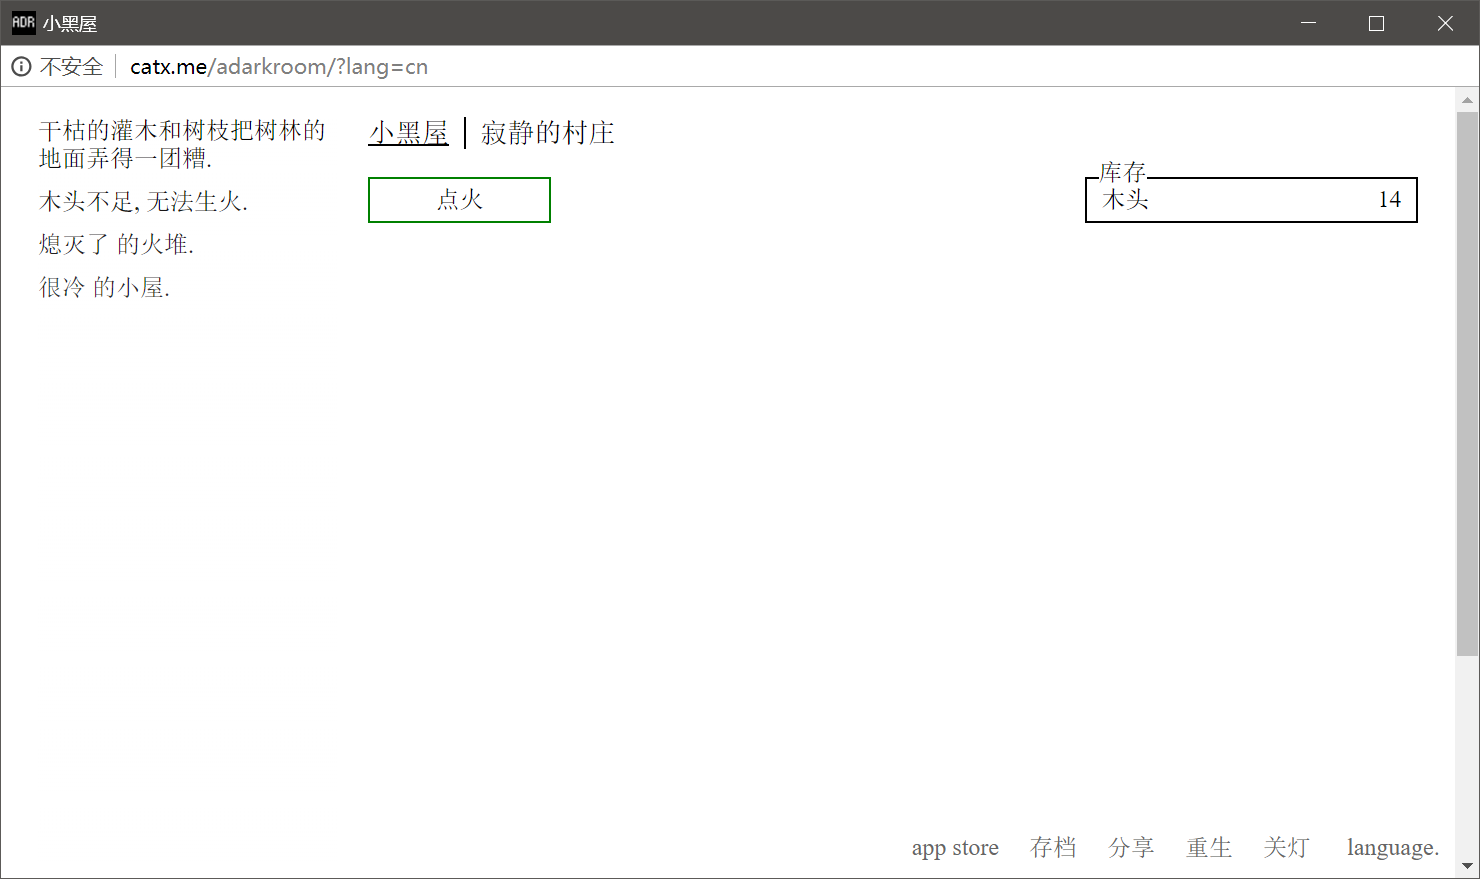
\includegraphics[width=0.9\textwidth]{adarkroom}
	\caption{「小黑屋」游戏画面}
	\label{fig:adarkroom}
\end{figure}

代码实现方面,尽管教学代码中使用了 C 语言,这里决定使用 C++ 来编写,得益于 C++ 的类机制和现代 C++ 的一些优质特性,程序会更加健壮、代码更加优雅。

\subsection{界面设计}

有了上小节所述的操作逻辑,开始思考界面设计。

为了保持视觉上的一致,加载界面不再使用和教学代码类似的设计,而是保持和后面的游戏界面同样的风格,在界面下方显示一个加载进度条滚动显示,如图 \ref{fig:loading_view}。加载完成后滚动条变为一个提示文字,提示用户按空格开始游戏。

\begin{figure}[htp]
	\centering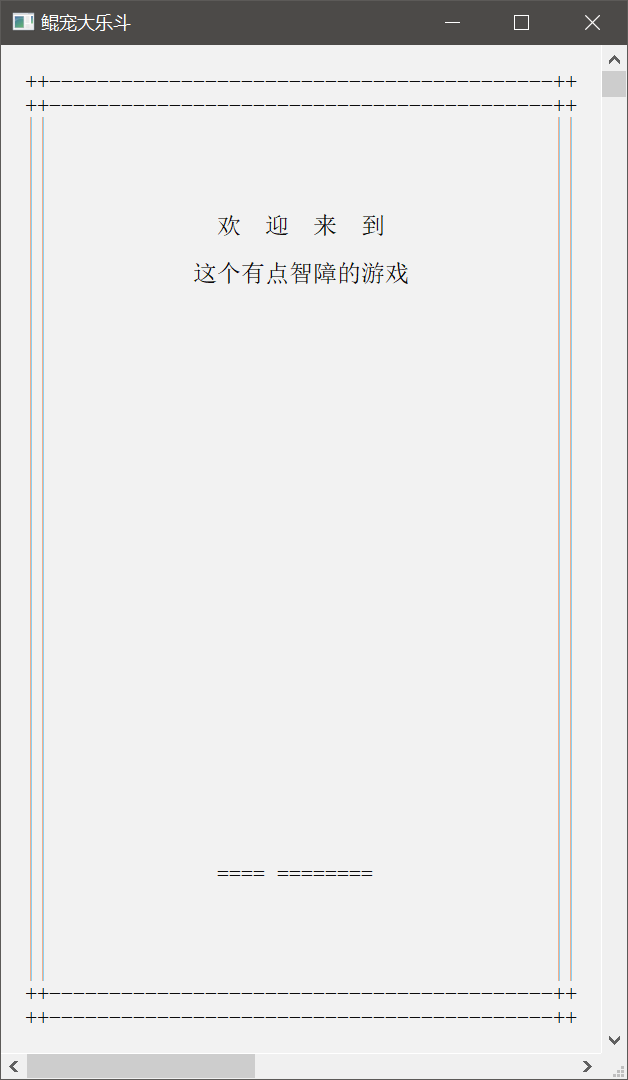
\includegraphics[width=0.5\textwidth]{loading_view}
	\caption{加载界面}
	\label{fig:loading_view}
\end{figure}

游戏界面方面,由于已经决定统一使用菜单进行功能的选择,那么整体只需要一种界面样式即可,界面边界处用字符画一个边框,界面上半部分显示可选的文本内容用于提示用户或显示游戏信息,下半部分显示游戏菜单,如图 \ref{fig:game_dashboard_view}。

\begin{figure}[htp]
	\centering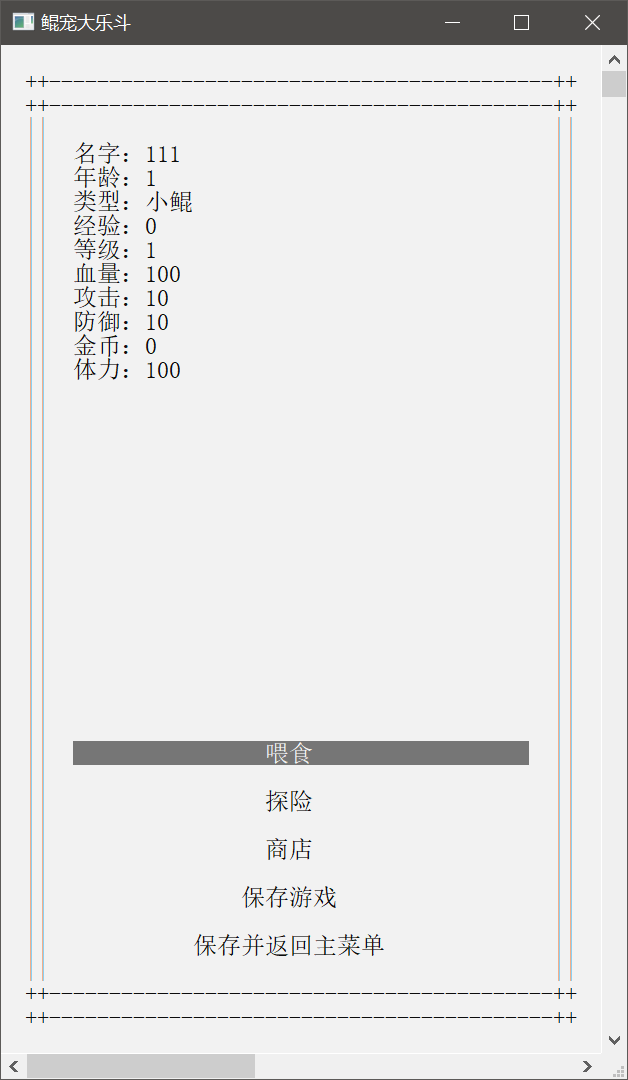
\includegraphics[width=0.5\textwidth]{game_dashboard_view}
	\caption{游戏界面的统一样式}
	\label{fig:game_dashboard_view}
\end{figure}

\subsection{体验设计}

游戏中宠物等级、升级机制、商店、战斗等涉及到游戏体验的内容,由小组其他成员设计,并在后续的代码实现过程中通过沟通交流进行了相应的扩展和妥协。

\subsection{程序架构设计}

前面的游戏逻辑和界面设计直接导致了程序架构将类似于桌面或手机应用软件,而非常见的基于物理引擎的视频游戏,经过一番考虑和妥协(由于时间相对比较紧迫,无法将其设计得过于复杂),决定从手机应用开发中借鉴\textbf{视图(View)}的概念(为了方便阅读,后面将主要使用「View」这一术语),抛去其中较为复杂且在此游戏中没有必要的 View 树机制(每个 View 中又可以包括各种子 View),而是简单地将一个游戏界面实现为一个 View,每个 View 直接占据全屏,View 之间的切换将直接覆盖掉当前界面,而不会保留上一层 View 所绘制的画面,当新的 View 退出、上一层 View 重新显示时,它将会重新绘制自身所需显示的内容。

有了 View 这样一个概念之后,可以将程序划分为四个模块:\codeinline{engine}、\codeinline{views}、\codeinline{core}、\codeinline{utils}。其中,\codeinline{engine} 模块实现了底层的界面绘制细节,并提供了几个基础的 \codeinline{View} 类;\codeinline{views} 模块中,每个游戏界面对应一个 \codeinline{View} 子类,用于实现游戏的操作逻辑;\codeinline{core} 模块提供了游戏的核心类,例如宠物类、战斗角色类、游戏存档和载入等;\codeinline{utils} 模块则提供零碎的、和主要程序不相关的辅助工具。下面将对这些模块的具体实现逐一做详细说明。

\subsection{程序实现}

\subsubsection{\codeinline{engine} 模块}

\codeinline{engine} 模块是整个游戏程序的基石,在程序架构设计得差不多之后,就需要开始实现此模块。

首先需要定义若干个与坐标和图形相关的基础类,具体而言包括 \codeinline{Point}、\codeinline{Size}、\codeinline{Rect}、\codeinline{Color},这些类定义在 \codeinline{types.h} 头文件中,依次分别表示坐标上的点(包括 X 和 Y 坐标)、大小范围(包括宽和高)、矩形(包括两个可以确定矩形位置和大小的顶点)、颜色。代码片段 \ref{snippet:size_class} 给出了 \codeinline{Size} 类的实现,其它类基本与其相似。

\begin{snippet}
	\cppfile{snippets/size_class.cpp}
	\caption{\codeinline{Size} 类的实现}
	\label{snippet:size_class}
\end{snippet}

然后在 \codeinline{engine.h} 头文件中定义了 \codeinline{Screen} 类,这个类封装了 Windows API 中对控制台的操作函数,对外提供了设置当前颜色、填充控制台一块矩形区域的颜色、从某一坐标开始打印字符串等接口,如代码片段 \ref{snippet:screen_class}。

\begin{snippet}
	\cppfile{snippets/screen_class.cpp}
	\caption{\codeinline{Screen} 类的实现}
	\label{snippet:screen_class}
\end{snippet}

由于 \codeinline{Screen} 类只是提供了一个基本的封装,对外提供的接口仍然较为底层,直接使用它来绘制 View 仍然较为麻烦,于是在它只上又封装了一个 \codeinline{Canvas} 类,该类内部保存一个 \codeinline{Screen} 类的引用,然后提供更为高层的接口,如绘制边框、在矩形范围内绘制文本(自动处理换行)、使用属性绘制文本(可设置对齐方式、边距大小等),代码片段 \ref{snippet:canvas_class} 展示了在矩形范围内绘制文本接口的实现。

\begin{snippet}
	\cppfile{snippets/canvas_class.cpp}
	\caption{\codeinline{Canvas} 类的在矩形范围内绘制文本接口}
	\label{snippet:canvas_class}
\end{snippet}

有了上面两个绘制相关的类之后,开始实现最重要的 \codeinline{View} 类,这个类虽然重要,但代码较为简单,主要就是定义了一个 View 的生命周期——何时被绘制、何时被重绘、何时进入主循环。\codeinline{View} 类是一个 \textbf{抽象基类},在实际使用时,会从它继承一个具体的类来绘制相应的游戏界面,代码片段 \ref{snippet:view_class} 展示了 \codeinline{View} 类的几个重要方法。

\begin{snippet}
	\cppfile{snippets/view_class.cpp}
	\caption{\codeinline{View} 类的几个重要方法}
	\label{snippet:view_class}
\end{snippet}

由于菜单是一个较为独立的组件,它有自己的特性,比如,需要在循环中接受用户的键盘输入、动态改变菜单项的高亮、在回车时执行不同的操作,实现中将它单独作为一个类来实现,即 \codeinline{Menu} 类。\codeinline{Menu} 类在每次循环开始的时候在给定的矩形范围内输出菜单项,并进入循环接收用户键盘输入,当收到键盘输入时,它会负责响应上下左右方向键,以上移或下移当前高亮的菜单项,而当输入是空格或回车时,它会调用创建菜单时传入的回调函数,并将当前选中的项的索引传入回调函数。\codeinline{Menu} 类的具体实现不再给出,相对的,代码片段 \ref{snippet:menu_view_class} 给出了在 \codeinline{View} 子类中使用 \codeinline{Menu} 类来输出菜单的一个例子——\codeinline{MenuView} 类的实现。

\begin{snippet}
	\cppfile{snippets/menu_view_class.cpp}
	\caption{\codeinline{MenuView} 类的实现}
	\label{snippet:menu_view_class}
\end{snippet}

\codeinline{MenuView}、\codeinline{TextView}、\codeinline{NoticeView} 是 \codeinline{engine} 模块提供的三个 \codeinline{View} 子类,分别用于提供显示菜单的视图、显示文本和菜单的视图、显示通知的视图(文本和仅有的一个菜单项)。利用这些预设的子类,游戏界面的实现将会更加简单方便。

\subsubsection{\codeinline{views} 模块}

该模块中全部是游戏界面的 View,例如 \codeinline{GameDashboardView}、\codeinline{AboutView}、\codeinline{BattleView} 等。它们全都继承自 \codeinline{View} 类或 \codeinline{engine} 模块预设的 \codeinline{View} 子类,然后覆盖父类的相应方法来实现不同的功能。以 \codeinline{BattleView} 为例,它继承自 \codeinline{TextView},覆盖了 \codeinline{std::string text()}、\codeinline{std::vector<std::string> menus()}、\codeinline{void on_select(Menu &menu, const int index)} 三个方法来分别定制界面上半部分显示的文本、界面下半部分显示的菜单项、选中菜单项之后的回调。得益于 \codeinline{View} 类和 \codeinline{TextView} 类的抽象,在 \codeinline{BattleView} 中完全不需要关注菜单如何显示、键盘如何选择等细节,而只需要专注于游戏控制逻辑的开发。

\subsubsection{\codeinline{core} 模块}

该模块提供游戏核心逻辑所需的类,由于这是一个宠物养成类的游戏,必须有一个类来表示宠物,其中包括宠物名字、年龄、等级、各种属性等,这些在 \codeinline{Pet} 类中定义。

除此之外该模块还提供了游戏存档和载入功能,以及战斗时的敌人和宠物两个角色的统一类 \codeinline{BattleSpirit}。

\subsubsection{游戏的启动}

总经过上面各模块的封装和抽象之后,启动游戏的代码如代码片段 \ref{snippet:start_game} 所示,优雅而美丽。

\begin{snippet}
	\cppfile{snippets/start_game.cpp}
	\caption{启动游戏的代码}
	\label{snippet:start_game}
\end{snippet}

\section{实习总结}

这五天的实习增进了自己对 Windows API 的熟悉和理解,对控制台字符界面程序有了新的体验,以前只是去用别人写的控制台程序,自己去实现的时候是有不一样的感受。另外,View 机制的实现也着实费了一些功夫,一方面,要实现得像手机应用那样复杂是没有时间和精力的,另一方面,如果完全不去做 View 机制,会使代码非常繁杂,不能很好的复用,从这里面的权衡之中还是有所收获的。

\section{思考与展望}

由于时间非常有限,虽说是五天实习,但实际开发时间只有两天左右,有很多细节考虑不是很到位,比如 \codeinline{Screen} 类和 \codeinline{Canvas} 类之间有很多功能上的重复,具体的接口设计也不是很明确区分,以及,View 的跳转机制虽然可以工作,但还是有些缺陷,如果要实现更复杂的界面,有可能还需要优化代码结构。

另外,大部分精力花在了程序架构上面,游戏实际功能做得比较少,有很多想法没有时间去落实。

以后如果有机会可以再次重新思考这样的程序的写法,实现一个更完善的试图机制,更可以实现一个物理引擎,这样它就同时具备了写类似应用的程序和类似游戏的程序的能力。

\end{document}
